\chapter{Geodesics} \label{s:geo}

\minitoc

\section{Introduction}

Geodesics play a key role in general relativity, since they represent
the worldlines of test particles, either massive or masseless (photons)
(cf. Sec.~\ref{s:fra:worldlines}). Moreover, for black hole theory,
null geodesics play a proeminant role, as the generators of the event horizons
(cf. Sec.~\ref{s:glo:properties_H}). We review here the definition and
properties of geodesics on a generic pseudo-Riemannian manifold.
Contrary to Appendix~\ref{s:bas}, proofs of the stated properties will be provided.

%%%%%%%%%%%%%%%%%%%%%%%%%%%%%%%%%%%%%%%%%%%%%%%%%%%%%%%%%%%%%%%%%%%%%%%%%%%%%%%

\section{Definition and first properties}

\subsection{Geodesics and affine parametrizations} \label{s:geo:def}

On a Riemannian manifold, i.e. a manifold equipped with a positive definite metric
(cf. Sec.~\ref{s:bas:signature}), a geodesic is the curve of minimal length between
two points (at least for close enough points). It is also a curve which is
``as straight as possible'', in the sense that its tangent vectors are transported parallelly
to themselves along it. A typical example is a geodesic in the Euclidean space: this is
necessarily a straight line; it is then obvious that its tangent vectors
keep a fixed direction. In a \emph{pseudo}-Riemannian manifold, such as the
spacetimes of general relativity, one uses
this last property to define geodesics:
\begin{greybox}
A smooth curve $\mathcal{C}$ of a pseudo-Riemannian manifold $(\M,\w{g})$ is
called a \defin{geodesic} iff it admits a parametrization $P$ whose associated
tangent vector field $\w{v}$ is transported parallelly to itself along
$\mathcal{C}$:
\be \label{e:geo:geod_eq_v}
    \encadre{\wnab_{\!\w{v}} \w{v} = 0},
\ee
where $\wnab$ is the Levi-Civita connection associated with $\w{g}$.
The parametrization $P$ is then called an
\defin{affine parametrization}\index{affine!parametrization}\index{parametrization!affine --}
and the corresponding parameter $\lambda$ is called an
\defin{affine paramater}\index{affine!parameter}\index{parameter!affine --} of the
geodesic $\mathcal{C}$. Note that the relation between $\w{v}$ and $\lambda$ is
\be \label{e:geo:v_dxdlambda}
    \w{v} = \frac{\D\w{x}}{\D\lambda} ,
\ee
where $\D\w{x}$ is the infinitesimal displacement along $\mathcal{C}$ corresponding
to the change $\D\lambda$ in the parameter $\lambda$
(cf. Eq.~(\ref{e:bas:dell_v_dlamb})).
\end{greybox}
In the above definition, let us recall that a \emph{curve}  is the image $\mathcal{C}=P(I)$
of a map (called a \emph{parametrization}) $P:\ I\rightarrow \M$,
where $I$ is an interval of $\R$, spanned by $\lambda$ (cf Sec.~\ref{s:bas:vectors}).
Moreover, we exclude the case where $\mathcal{C}$ is reduced to a single point
of $\M$, i.e. where $P$ is a constant function.

The qualifier \emph{affine} in the above definition stems from the following
property:
\begin{greybox}
Any two affine parametrizations of a geodesic $\mathcal{C}$ are necessarily
related by an affine transformation:
\be \label{e:geo:affine_transf}
    \lambda' = a \lambda + b,
\ee
where $a$ and $b$ are two real constants such that $a\not = 0$.
\end{greybox}
\begin{proof}
Let $P: I \to  \mathcal{C}\subset\M$, $\lambda\mapsto P(\lambda)$ and
$P': I'\to \mathcal{C}$,
$\lambda'\mapsto P'(\lambda')$ be two
parametrizations of $\mathcal{C}$. They are necessarily related by a
diffeomorphism $I\to I'$, $\lambda \mapsto \lambda'(\lambda)$. It follows
from Eq.~(\ref{e:geo:v_dxdlambda}) that the tangent vector fields $\w{v}$ and $\w{v'}$
associated with these two parametrizations are related by
\be  \label{e:geo:change_tangent_vector}
    \w{v} = \frac{\D\lambda'}{\D\lambda} \, \w{v'} .
\ee
Using the rules 2 and 3 governing the connection $\wnab$ (cf. Sec.~\ref{s:bas:affine_connect}),
we get then
\be \label{e:geo:acc_v_acc_vp}
    \wnab_{\!\w{v}}\w{v} = \frac{\D^2\lambda'}{\D\lambda^2} \, \w{v'}
    + \left( \frac{\D\lambda'}{\D\lambda} \right)^2 \wnab_{\!\w{v'}}\w{v'} .
\ee
If both parametrizations are affine, then $\wnab_{\!\w{v}}\w{v} = 0$ and
$\wnab_{\!\w{v'}}\w{v'} = 0$, so that the above identity reduces to
${\D^2\lambda'}/{\D\lambda^2} = 0$, which implies
the affine law (\ref{e:geo:affine_transf}).
\end{proof}

\begin{remark}
Because of (\ref{e:geo:geod_eq_v}), a geodesic is also called
an \defin{autoparallel curve}\index{autoparallel}. It is also sometimes called
a \defin{zero-acceleration curve}\index{zero-acceleration}, the
vector $\wnab_{\!\w{v}}\w{v}$ being considered as the
``acceleration''\index{acceleration! of a curve} of (the parametrization $P$ of) the
curve $\mathcal{C}$; this is of course by extension of the concept of
4-acceleration $\w{a} := \wnab_{\!\w{u}}\w{u}$ of a timelike worldline
with 4-velocity $\w{u}$, the latter being nothing but the tangent vector associated with
the parametrization of the worldline by its proper time.
\end{remark}

An important property of geodesics is
\begin{greybox}
Let $\mathcal{C}$ be a geodesic of $(\M,\w{g})$ and $\w{v}$ a tangent vector field
associated with an affine parametrization of $\mathcal{C}$. Then the
scalar square of $\w{v}$ with respect to the metric $\w{g}$
is constant along $\mathcal{C}$:
\be \label{e:geo:vv_const}
    \w{g}(\w{v},\w{v}) = \mathrm{const}.
\ee
\end{greybox}
\begin{proof}
The variation of $\w{g}(\w{v},\w{v})$ along $\mathcal{C}$ is given
by
\bea
 \wnab_{\!\w{v}} \left[ \w{g}(\w{v},\w{v}) \right] & = & v^\mu \nabla_\mu (g_{\rho\sigma} v^\rho v^\sigma) \nonumber \\
            & = & v^\mu \underbrace{\nabla_\mu g_{\rho\sigma}}_{0} v^\rho v^\sigma
                + g_{\rho\sigma} \underbrace{v^\mu \nabla_\mu v^\rho}_{0} v^\sigma
                + g_{\rho\sigma} v^\rho \underbrace{v^\mu \nabla_\mu v^\sigma}_{0} = 0 , \nonumber
\eea
where we have used the facts that $\wnab$ is the Levi-Civita connection of $\w{g}$ [Eq.~(\ref{e:bas:nabla_g_zero})] and $\w{v}$ obeys the geodesic equation (\ref{e:geo:geod_eq_v}).
\end{proof}
For a Lorentzian manifold, the constancy of $\w{g}(\w{v},\w{v})$ has an
interesting corollary: the tangent vector $\w{v}$ cannot change its type
along $\mathcal{C}$. Hence:
\begin{greybox}
In a Lorentzian manifold $(\M,\w{g})$, a geodesic $\mathcal{C}$ belongs necessarily
to one of the following three categories:
\begin{itemize}
\item \defin{timelike geodesic}\index{timelike!geodesic}\index{geodesic!timelike --}:
tangent vectors are timelike at all points of $\mathcal{C}$;
\item \defin{null geodesic}\index{null!geodesic}\index{geodesic!null --}:
tangent vectors are null at all points of $\mathcal{C}$;
\item \defin{spacelike geodesic}\index{spacelike!geodesic}\index{geodesic!spacelike --}:
tangent vectors are spacelike at all points of $\mathcal{C}$.
\end{itemize}
\end{greybox}
This is in sharp contrast with generic curves, which can be, for instance, timelike on some portions
and null or spacelike on other parts.

In the timelike case, or the spacelike one,
the tangent vector field $\w{v}$ can be rescaled by the constant $\sqrt{|\w{g}(\w{v},\w{v})|}$ to get
a unit tangent vector field, i.e. a tangent vector field $\w{u}$ which obeys
$\w{g}(\w{u},\w{u}) = -1$ (timelike geodesic) or $\w{g}(\w{u},\w{u}) = 1$
(spacelike geodesic). Moreover, in doing so, the affine character of the
parametrization is preserved. Indeed, the rescaling amounts to choosing the constant $a$
in the affine law~(\ref{e:geo:affine_transf}) such that $a = \sqrt{|\w{g}(\w{v},\w{v})|}$.
Thus, we have
\begin{greybox}
A timelike or spacelike geodesic of a Lorentzian manifold has an affine parametrization,
the tangent vector of which is a unit vector (i.e. of scalar square $\pm 1$ with respect to
$\w{g}$). Moreover this parametrization is unique up to some choice of origin
(choice of $b$ in (\ref{e:geo:affine_transf})) and of
orientation ($a=\pm 1$ in (\ref{e:geo:affine_transf})).
\end{greybox}
We shall see in Sec.~\ref{s:geo:gener_param} that for a timelike geodesic,
the affine parameter with unit tangent vector is nothing but the
\emph{proper time}\index{proper!time}\index{time!proper --}, while for a spacelike
geodesic, it is the \emph{arc length}\index{arc length}.

\subsection{Generic parametrizations of geodesics} \label{s:geo:gener_param}

Geodesics can be characterized by any of their tangent vectors, i.e.
tangent vectors not necessarily associated with an affine parametrization, as follows:
\begin{greybox}
A curve $\mathcal{C}$ is a geodesic
iff the tangent vector field $\w{v}$ associated with any parametrization
of $\mathcal{C}$ obeys
\be \label{e:geo:v_pregeodesic}
    \wnab_{\!\w{v}}\w{v} = \kappa\,  \w{v},
\ee
where $\kappa$ is a scalar field along $\mathcal{C}$.
\end{greybox}
\begin{proof}
Let $P: I\to \mathcal{C}$, $\lambda\mapsto P(\lambda)$ be the parametrization of $\mathcal{C}$
corresponding to the tangent vector field $\w{v}$: $\w{v} = \D\w{x}/\D\lambda$.
If $\mathcal{C}$ is a geodesic, then there exists a parametrization
$\lambda'\mapsto P'(\lambda')$ whose tangent vector, $\w{v'}$ say, obeys
$\wnab_{\!\w{v'}}\w{v'} = 0$. Since any two parametrizations of $\mathcal{C}$
are related by Eq.~(\ref{e:geo:acc_v_acc_vp}), we deduce that $\w{v}$ obeys
(\ref{e:geo:v_pregeodesic}) with
\[
    \kappa = \left( \frac{\D\lambda'}{\D\lambda} \right)^{-1}
        \frac{\D^2\lambda'}{\D\lambda^2} .
\]
Conversely, if $\w{v}$ obeys (\ref{e:geo:v_pregeodesic}) with $\kappa=\kappa(\lambda)$,
then Eq.~(\ref{e:geo:acc_v_acc_vp}) implies that $\wnab_{\!\w{v'}}\w{v'} = 0$,
i.e. that $\mathcal{C}$ is a geodesic, provided that the change of
parametrization $\lambda' = \lambda'(\lambda)$ fulfills
\[
    \kappa(\lambda) \frac{\D\lambda'}{\D\lambda} -  \frac{\D^2\lambda'}{\D\lambda^2} = 0 .
\]
This differential equation has the following solution:
\[
    \lambda' = a \int_{\lambda_1}^\lambda \left[ \exp \left(
    \int_{\lambda_0}^{\tilde{\lambda}} \kappa(\tilde{\tilde{\lambda}})
    \D\tilde{\tilde{\lambda}}\right) \D\tilde\lambda
    \right] + b,
\]
where $a$, $b$, $\lambda_0$ and $\lambda_1$ are constants, with $a\not = 0$ and $\lambda_0,\lambda_1\in I$.
\end{proof}
The above property motivates the following definitions:
\begin{greybox}
A vector field $\w{v}$ obeying (\ref{e:geo:v_pregeodesic}) is called
a \defin{pregeodesic vector field}\index{pregeodesic vector field}.
The scalar field $\kappa$ is then called the \defin{non-affinity coefficient}\index{non-affinity coefficient} of $\w{v}$.
If $\kappa=0$, $\w{v}$ is naturally called a \defin{geodesic vector field}\index{geodesic!vector field}.
\end{greybox}
Note that the property established above is equivalent to stating that the
field lines of a pregeodesic vector field are geodesics.

An easy consequence of Eq.~(\ref{e:geo:v_pregeodesic}) is the following
evolution law for the scalar square of the tangent vector:
\begin{greybox}
Along a geodesic $\mathcal{C}$, the scalar square $\w{g}(\w{v},\w{v})$
of the tangent vector $\w{v}$ associated with any parametrization of $\mathcal{C}$
evolves according to
\be \label{e:geo:evol_vv_kappa}
    \wnab_{\!\w{v}} \left[ \w{g}(\w{v},\w{v}) \right] = 2 \kappa \, \w{g}(\w{v},\w{v}),
\ee
where $\kappa$ is the non-affinity coefficient of $\w{v}$.
\end{greybox}
\begin{proof}
One has, using $\wnab\w{g}=0$ [Eq.~(\ref{e:bas:nabla_g_zero})] and Eq.~(\ref{e:geo:v_pregeodesic}),
\[
    v^\mu \nabla_\mu (g_{\rho\sigma} v^\rho v^\sigma)  = v^\mu \underbrace{\nabla_\mu g_{\rho\sigma}}_{0} v^\rho v^\sigma
                + g_{\rho\sigma} \underbrace{v^\mu \nabla_\mu v^\rho}_{\kappa v^\rho} v^\sigma
                + g_{\rho\sigma} v^\rho \underbrace{v^\mu \nabla_\mu v^\sigma}_{\kappa v^\sigma}
             = 2 \kappa  g_{\rho\sigma} v^\rho v^\sigma  ,
\]
hence the law (\ref{e:geo:evol_vv_kappa}).
\end{proof}
We recover of course (\ref{e:geo:vv_const}) in the special case $\kappa = 0$
($\w{v}$ geodesic vector).
\begin{remark}
If $\lambda$ is the parameter associated with $\w{v}$: $\w{v} = \D\w{x}/\D\lambda$,
we may introduce the scalar function $V(\lambda) := \w{g}(\w{v},\w{v})$ and
rewrite (\ref{e:geo:evol_vv_kappa}) as a first-order ordinary differential equation
for it [cf. Eq.~(\ref{e:bas:def_vector})]:
\be
    \frac{\D V}{\D\lambda} = 2 \kappa(\lambda) V(\lambda) .
\ee
\end{remark}
A consequence of (\ref{e:geo:evol_vv_kappa}) is
\begin{greybox}
On a Lorentzian manifold, the parametrization of a timelike geodesic
by the proper time\index{time!proper --} ($\lambda = \tau$) is an affine parametrization.
Similarly, on a Lorentzian or Riemannian manifold, the parametrization of a
spacelike geodesic
by the arc length\index{arc length} ($\lambda = s$) is an affine parametrization.
\end{greybox}
\begin{proof}
The tangent vector associated with the proper time $\tau$ along a timelike geodesic
is nothing but the 4-velocity $\w{u}$ (cf. Sec.~\ref{s:fra:massive_part}), which
is of constant scalar square: $\w{g}(\w{u},\w{u}) = -1$, so that Eq.~(\ref{e:geo:evol_vv_kappa})
reduces to $0 = -2 \kappa$, hence $\kappa=0$, which implies that we are dealing
with an affine parametrization. Similarly, the tangent vector associated with the
arc length $s$ along a spacelike geodesic has a scalar square everywhere equal
to 1, leading to the same conclusion.
\end{proof}

%%%%%%%%%%%%%%%%%%%%%%%%%%%%%%%%%%%%%%%%%%%%%%%%%%%%%%%%%%%%%%%%%%%%%%%%%%%%%%%

\section{Existence and uniqueness of geodesics}

\subsection{The geodesic equation}

\begin{greybox}
Let $\mathcal{C}$ be a curve in a pseudo-Riemannian
manifold $(\M,\w{g})$ of dimension $n$, such that
$\mathcal{C}$ is contained in the domain of a coordinate chart $(x^\alpha)_{0\leq\alpha\leq n-1}$.
Then any parametrization of $\mathcal{C}$, $P: I \to  \mathcal{C}$, $\lambda\mapsto P(\lambda)$,
can be described by $n$ functions $X^\alpha: I\to \R$
according to Eq.~(\ref{e:bas:curve_param_equation}): $x^\alpha(P(\lambda)) = X^\alpha(\lambda)$.
The curve $\mathcal{C}$ is a geodesic iff there exists a paramatrization of $\mathcal{C}$
for which the functions $X^\alpha$ fullfills the following
system of $n$ second-order differential equations, usually called the
\defin{geodesic equation}\index{geodesic!equation}\index{equation!geodesic --}:
\be \label{e:geo:eq_geod}
    \encadre{ \frac{\D^2 X^\alpha}{\D\lambda^2} + \Gamma^\alpha_{\ \, \mu \nu}
    \frac{\D X^\mu}{\D\lambda} \frac{\D X^\nu}{\D\lambda} = 0 },  \qquad 0 \leq \alpha \leq n-1,
\ee
where the $\Gamma^\alpha_{\ \, \mu \nu}$'s are the Christoffel symbols\index{Christoffel symbols} of the metric $\w{g}$
with respect to the coordinates $(x^\alpha)$, as given by Eq.~(\ref{e:bas:Christoffel}).
\end{greybox}
\begin{proof}
Notice first that the components with respect
to the chart $(x^\alpha)$ of the tangent
vector field $\w{v}$ associated with the parameter $\lambda$ are [cf. Eq.~(\ref{e:bas:va_dXadlamb})]
\be \label{e:geo:va_dXadlamb}
    v^\alpha = \frac{\D X^\alpha}{\D\lambda} .
\ee
On the other side, the components of $\wnab_{\!\w{v}}\w{v}$ are
\[
    v^\mu \nabla_\mu v^\alpha = v^\mu \der{v^\alpha}{x^\mu} + \Gamma^\alpha_{\ \, \mu \nu} v^\mu v^\nu
    = \w{v}(v^\alpha) + \Gamma^\alpha_{\ \, \mu \nu} v^\mu v^\nu
    = \frac{\D v^\alpha}{\D \lambda} + \Gamma^\alpha_{\ \, \mu \nu} v^\mu v^\nu ,
\]
where we have used
successively Eqs.~(\ref{e:bas:der_cov_coord}), (\ref{e:bas:v_va_wpar_a}) and
(\ref{e:bas:def_vector}). The above relation, along with (\ref{e:geo:va_dXadlamb}),
shows that the left-hand side of
Eq.~(\ref{e:geo:eq_geod}) is nothing but the component $\alpha$ of
$\wnab_{\!\w{v}}\w{v}$. The conclusion follows from the very definition
of a geodesic given in Sec.~\ref{s:geo:def}.
\end{proof}

Note that if a solution of the geodesic equation (\ref{e:geo:eq_geod}) is found, the parameter
$\lambda$ is necessarily an affine parameter.
For a generic parameter,
the differential equation becomes (\ref{e:geo:eq_geod}) with the right-hand side
replaced by $\kappa \D X^\alpha /\D\lambda$, which is the coordinate
expression of the right-hand side $\kappa \w{v}$ in
Eq.~(\ref{e:geo:v_pregeodesic}). Hence, we have
\begin{greybox}
A curve $\mathcal{C}$ in the domain of a chart $(x^\alpha)$ is a geodesic
iff some (actually all) coordinate expression $x^\alpha = X^\alpha(\lambda)$
of $\mathcal{C}$ fulfills the following
system of $n$ second-order differential equations, usually called the
\defin{pregeodesic equation}\index{pregeodesic!equation}\index{equation!pregeodesic --},
\be \label{e:geo:pregeod_eq_comp}
    \encadre{ \frac{\D^2 X^\alpha}{\D\lambda^2} + \Gamma^\alpha_{\ \, \mu \nu}
    \frac{\D X^\mu}{\D\lambda} \frac{\D X^\nu}{\D\lambda} =
    \kappa(\lambda) \frac{\D X^\alpha}{\D\lambda}   },  \qquad 0 \leq \alpha \leq n-1 .
\ee
for some real-valued function $\kappa(\lambda)$.
\end{greybox}

\subsection{Existence and uniqueness}

We may use the geodesic equation to prove the following existence and uniqueness
theorem:
\begin{greybox}
Given a point $p$ in a pseudo-Riemannian manifold $(\M,\w{g})$ and a vector
$\w{V}$ in the tangent space to $\M$ at $p$, i.e. $\w{V} \in T_p\M$,
there exists a geodesic $\mathcal{C}$ through $p$ such that
$\w{V}$ is the value at $p$ of the tangent vector of some affine parametrization
of $\mathcal{C}$:
\be
    \w{V} = \left. \frac{\D\w{x}}{\D\lambda} \right|_p .
\ee
Morever, this geodesic is unique, in the sense that any geodesic $\mathcal{C}'$
sharing the same property coincides with $\mathcal{C}$
in some open neighbourhood of $p$.
\end{greybox}
\begin{proof}
Let $(x^\alpha)$ be a coordinate chart of $\M$ around $p$. Let $(V^\alpha)$
be the component of $\w{V}$ in the basis of $T_p\M$ induced by
the coordinate frame $(\wpar_\alpha)$ associated with $(x^\alpha)$:
\[
    \w{V} = V^\alpha \left. \wpar_\alpha \right| _p .
\]
A geodesic through $p$ having $\w{V}$ as tangent vector at $p$ is then
obtained as a solution $(X^\alpha(\lambda))$ of the system (\ref{e:geo:eq_geod})
with the initial conditions [cf. Eq.~(\ref{e:geo:va_dXadlamb})]
\be \label{e:geo:init_cond}
    X^\alpha(0) = x^\alpha(p) \quad\mbox{and}\quad
    \frac{\D X^\alpha}{\D\lambda}(0) = V^\alpha .
\ee
The system (\ref{e:geo:eq_geod}) + (\ref{e:geo:init_cond}) constitutes a well-posed
Cauchy problem\index{Cauchy problem} and standard results about ordinary
differential equations, e.g. the Picard-Lindelöf (or Cauchy–Lipschitz) theorem,
guarantee the existence and uniqueness of the solution.
\end{proof}

A few definitions are in order:

\begin{greybox}
A geodesic $\mathcal{C}$ is said to be \defin{maximal}\index{maximal!geodesic}\index{geodesic!maximal --}
or \defin{inextendible}\index{inextendible geodesic}\index{geodesic!inextendible --} iff
there does not exist any geodesic $\mathcal{C}'$ such that  $\mathcal{C}\subset\mathcal{C}'$ and
$\mathcal{C}'\not=\mathcal{C}$.
\end{greybox}

\begin{greybox}
A geodesic $\mathcal{C}$ is \defin{complete}\index{complete!geodesic}\index{geodesic!complete --}
iff it is maximal and the interval spanned by any of its affine parameters is the whole real line:
$I=\R$. The pseudo-Riemannian manifold $(\M,\w{g})$ is said to be \defin{geodesically complete}
iff every maximal geodesic is complete.
\end{greybox}

\begin{remark}
A well-known theorem of differential geometry, namely the \defin{Hopf-Rinow theorem}\index{Hopf-Rinow theorem},
states that a connected \emph{Riemannian} manifold is geodesically complete iff it is \emph{complete}
as a \emph{metric space}\index{metric!space} for the distance function $d(p,q)$ defined as the infimum of
the metric length of all curves connecting the two points $p$ and $q$
(see e.g. Ref.~\cite{Lee97}). However, there is no such theorem for \emph{Lorentzian}
manifolds, for the metric does not induce any distance function turning them into a metric space.
\end{remark}


We have the following proposition, strengthening the existence and uniqueness
result obtained above:
\begin{greybox}
Given a point $p$ in a pseudo-Riemannian manifold $(\M,\w{g})$ and a vector
$\w{V}$ in the tangent space to $\M$ at $p$, i.e. $\w{V} \in T_p\M$,
there exists a unique maximal geodesic through $p$, which we shall denote
by $\mathcal{C}_{\w{V}}$, such that
$\w{V}$ is the value at $p$ of the tangent vector of some affine parametrization
of $\mathcal{C}_{\w{V}}$. We shall then denote by $P_{\w{V}}$ the unique
affine parametrization of $\mathcal{C}_{\w{V}}$ such that
\be
    P_{\w{V}}(0) = p \quad\mbox{and}\quad \left.\w{v}\right| _p = \w{V} ,
\ee
where $\w{v}$ is the tangent vector of
$P_{\w{V}}$.
\end{greybox}
We refer to O'Neill's textbook \cite{ONeil83}, p.~68 for the proof.

\subsection{Exponential map}

\begin{greybox}
Given a point $p$ in a pseudo-Riemannian manifold $(\M,\w{g})$,
let $\mathcal{E}_p$ be the subset of the tangent space $T_p\M$ defined
by $\w{V}\in \mathcal{E}_p$ iff the affine parametrization $P_{\w{V}}$
of the geodesic $\mathcal{C}_{\w{V}}$, whose tangent vector coincides
with $\w{V}$ at $p$, has a domain large enough to include the interval $[0,1]$.
The \defin{exponential map at $p$}\index{exponential map} is then defined as
\be
    \begin{array}{cccc}
    \exp_p : & \mathcal{E}_p \subset T_p\M & \longrightarrow & \M \\
    & \w{V} & \longmapsto & P_{\w{V}}(1) .
    \end{array}
\ee
\end{greybox}
Note that if $(\M,\w{g})$ is geodesically complete, $\mathcal{E}_p = T_p\M$
for every point $p$.


%%%%%%%%%%%%%%%%%%%%%%%%%%%%%%%%%%%%%%%%%%%%%%%%%%%%%%%%%%%%%%%%%%%%%%%%%%%%%%%

\section{Geodesics and variation of length}

\subsection{Length of a curve}

Here, we make some attempt to connect geodesics in a pseudo-Riemannian manifold
with the first feature mentioned in Sec.~\ref{s:geo:def}, namely geodesics are
locally the curves of \emph{minimal length} in a Riemannian manifold.
We have first to define the length of a curve.
Of course, when the metric is not definite positive, one cannot use
the integral of the norm of infinitesimal displacements along the curve,
i.e. $\D s := \sqrt{\w{g}(\D\w{x},\D\w{x})}$, since $\w{g}(\D\w{x},\D\w{x})$
can be negative. Rather, one defines the length from
$\D s := \sqrt{|\w{g}(\D\w{x},\D\w{x})|}$. Using $\D\w{x} = \w{v}\D \lambda$
[Eq.~(\ref{e:bas:dell_v_dlamb})], we end up with the following definition.
\begin{greybox}
The \defin{length}\index{length!of a curve} of a curve
$\mathcal{C}$ connecting two points $p$ and $q$
in a pseudo-Riemannian manifold $(\M,\w{g})$ is
\be \label{e:geo:def_length}
    L_{(p,q)}(\mathcal{C}) := \int_{\lambda_p}^{\lambda_q} \sqrt{\left|
        \w{g}(\w{v},\w{v}) \right| } \, \D\lambda ,
\ee
where $\lambda$ is some parameter along $\mathcal{C}$, $\lambda_p$
(resp. $\lambda_q$) being its value at $p$ (resp. $q$),
$\w{v} = \D\w{x}/\D\lambda$ is the associated tangent vector field,
and we assume $\lambda_q \geq \lambda_p$.
\end{greybox}
Thanks to the transformation law (\ref{e:geo:change_tangent_vector}), it is
easy to check that the value of $L_{(p,q)}(\mathcal{C}) $ is independent from
the choice of the parametrization of $\mathcal{C}$, i.e. for a fixed
pair of points $(p,q)$, it is a function of $\mathcal{C}$ only.

When $\mathcal{C}$ is included in the domain of a coordinate chart
$(x^\alpha)$, so that its equation is $x^\alpha = X^\alpha(\lambda)$, we
may rewrite (\ref{e:geo:def_length}) as [cf. Eq.~(\ref{e:geo:va_dXadlamb})]
\be \label{e:geo:def_length_X}
    L_{(p,q)}(\mathcal{C})  := \int_{\lambda_p}^{\lambda_q} \sqrt{\left|
        g_{\mu\nu}(X^\rho(\lambda)) \frac{\D X^\mu}{\D\lambda}
            \frac{\D X^\nu}{\D\lambda}\right| } \, \D\lambda ,
\ee
where $g_{\mu\nu}(X^\rho(\lambda))$ stands for the components of the
metric tensor $\w{g}$ with respect to the coordinates $(x^\alpha)$ at the
point of coordinates $X^\rho(\lambda)$.

\subsection{Timelike and spacelike geodesics as stationary points
of the length functional}

To find the curves connecting $p$ and $q$ of extremal length, it is
quite natural to study the behaviour of the length as a
variational problem, i.e. consider $L_{(p,q)}(\mathcal{C})$ as an ``action''
and write the Euler-Lagrange equation
for the ``Lagrangian'' defined as the integrand of (\ref{e:geo:def_length_X}):
\be \label{e:geo:Lagrangian}
    \mathcal{L}(X^\alpha, \dot{X}^\alpha) = \sqrt{\left|
        g_{\mu\nu}(X^\rho) \dot{X}^\mu \dot{X}^\nu \right| },
\ee
where we have introduced the standard dot notation for the ``velocity'' variables:
$\dot{X}^\alpha := \D X^\alpha / \D\lambda$. Before proceeding, a few
caveats must be made. First of all, the Euler-Lagrange equation
locate only \emph{stationary} points of the action (here the length
$L_{(p,q)}(\mathcal{C})$), i.e. points where the action does not vary
to first order in small changes of the curve. Such points are not
necessarily extrema: they can be \emph{saddle} points, as we shall see.
Secondly, because of the square root in (\ref{e:geo:Lagrangian}),
the Lagrangian is not differentiable at points where
$g_{\mu\nu} \dot{X}^\mu \dot{X}^\nu = 0$.
This corresponds to points where the curve $\mathcal{C}$ is null. We shall
therefore exclude such curves in our analysis (we shall return to null
curves later on). But then $g_{\mu\nu} \dot{X}^\mu \dot{X}^\nu$
has to be either always positive along $\mathcal{C}$ (i.e. $\mathcal{C}$
is spacelike) or always negative (i.e. $\mathcal{C}$ is timelike); indeed,
by continuity it cannot change sign without going through zero.
We shall then apply the variational principle separately
to two subsets of curves connecting $p$ and $q$: the timelike ones and the
spacelike ones. The calculations can be conducted in parallel by introducing
a sign parameter: $\eps=-1$ for timelike curves and $\eps=+1$ for spacelike
ones. One can then get rid of the absolute value in the Lagrangian, which
becomes
\be \label{e:geo:Lagrangian_eps}
    \mathcal{L}(X^\alpha, \dot{X}^\alpha) = \sqrt{\eps
        g_{\mu\nu}(X^\rho) \dot{X}^\mu \dot{X}^\nu  } .
\ee
Asking that the length (\ref{e:geo:def_length_X}) is stationary
with respect to small changes in the curve connecting $p$ and $q$
is equivalent to the Euler-Lagrange equation:
\be \label{e:geo:Euler-Lagrange}
    \frac{\D}{\D\lambda}\left( \der{\mathcal{L}}{\dot{X}^\alpha}\right)
        - \der{\mathcal{L}}{X^\alpha} = 0 .
\ee
We have
\[
    \der{}{X^\alpha} \left( g_{\mu\nu}(X^\rho) \dot{X}^\mu \dot{X}^\nu \right)
        = \der{g_{\mu\nu}}{x^\alpha}  \dot{X}^\mu \dot{X}^\nu  ,
\]
with the understanding that $\dert{g_{\mu\nu}}{x^\alpha}$ shall be
taken at the point $X^\rho(\lambda)$. Hence, given the Lagrangian (\ref{e:geo:Lagrangian_eps}),
\be \label{e:geo:derL_X}
  \der{\mathcal{L}}{X^\alpha} = \frac{\eps}{2\mathcal{L}} \der{g_{\mu\nu}}{x^\alpha}  \dot{X}^\mu \dot{X}^\nu .
\ee
Besides,
\[
    \der{}{\dot{X}^\alpha} \left( g_{\mu\nu}(X^\rho) \dot{X}^\mu \dot{X}^\nu \right)
        = g_{\alpha\nu} \dot{X}^\nu + g_{\mu\alpha} \dot{X}^\mu
        = 2 g_{\alpha\mu} \dot{X}^\mu .
\]
Hence
\[
    \der{\mathcal{L}}{\dot{X}^\alpha} = \frac{\eps}{\mathcal{L}} g_{\alpha\mu} \dot{X}^\mu  ,
\]
from which,
\be \label{e:geo:derL_Xdot}
    \frac{\D}{\D\lambda}\left( \der{\mathcal{L}}{\dot{X}^\alpha}\right) =
      - \frac{\eps}{\mathcal{L}^2}  \frac{\D \mathcal{L}}{\D\lambda} g_{\alpha\mu} \dot{X}^\mu
      + \frac{\eps}{\mathcal{L}} \der{g_{\alpha\mu}}{x^\nu} \dot{X}^\nu \dot{X}^\mu
      + \frac{\eps}{\mathcal{L}} g_{\alpha\mu} \ddot{X}^\mu .
\ee
In view of (\ref{e:geo:derL_X}) and (\ref{e:geo:derL_Xdot}), the
Euler-Lagrange equation (\ref{e:geo:Euler-Lagrange}) becomes
\[
  - \frac{1}{\mathcal{L}}  \frac{\D \mathcal{L}}{\D\lambda} g_{\alpha\mu} \dot{X}^\mu
      + \der{g_{\alpha\mu}}{x^\nu} \dot{X}^\mu \dot{X}^\nu
      +  g_{\alpha\mu} \ddot{X}^\mu
    - \frac{1}{2} \der{g_{\mu\nu}}{x^\alpha}  \dot{X}^\mu \dot{X}^\nu = 0 .
\]
Now, playing with the names of repeated indices and using the symmetry
of $g_{\alpha\beta}$, we can rewrite the second term as
\[
    \der{g_{\alpha\mu}}{x^\nu} \dot{X}^\mu \dot{X}^\nu
    = \frac{1}{2} \left( \der{g_{\alpha\nu}}{x^\mu} \dot{X}^\nu \dot{X}^\mu
    + \der{g_{\mu\alpha}}{x^\nu} \dot{X}^\mu \dot{X}^\nu \right)
    = \frac{1}{2} \left( \der{g_{\alpha\nu}}{x^\mu}
    + \der{g_{\mu\alpha}}{x^\nu} \right) \dot{X}^\mu \dot{X}^\nu .
\]
Accordingly, we get
\be \label{e:geo:geod_eq_cov}
    g_{\alpha\mu} \ddot{X}^\mu + \frac{1}{2} \left( \der{g_{\alpha\nu}}{x^\mu}
    + \der{g_{\mu\alpha}}{x^\nu} - \der{g_{\mu\nu}}{x^\alpha} \right) \dot{X}^\mu \dot{X}^\nu
    = \kappa g_{\alpha\mu} \dot{X}^\mu ,
\ee
where we have introduced
\[
    \kappa := \frac{1}{\mathcal{L}}  \frac{\D \mathcal{L}}{\D\lambda} .
\]
If we multiply Eq.~(\ref{e:geo:geod_eq_cov}) by the matrix $g^{\alpha\beta}$
(the components of the inverse metric) and use
$g^{\alpha\beta} g_{\alpha\mu} = \delta^\beta_{\ \, \mu}$ as well as
the expression (\ref{e:bas:Christoffel}) of the Christoffel symbols,
we get exactly the pregeodesic equation (\ref{e:geo:pregeod_eq_comp}).
Hence we conclude
\begin{greybox}
Among all the timelike (resp. spacelike) curves connecting two points $p$ and $q$, a curve has
a stationary length iff it is a timelike (resp. spacelike) geodesic.
\end{greybox}

For a timelike geodesic, and for points $p$ and $q$ not too far,
the stationary length corresponds to a \emph{maximum}: any other timelike curve
connecting $p$ and $q$ has a smaller length. If one interprets timelike
curves as worldlines and the length as the proper time, the above maximum
is nothing but a generalization of the standard ``twin paradox''\index{twin paradox}
of special relativity, as the example below illustrates.

\begin{figure}
\centerline{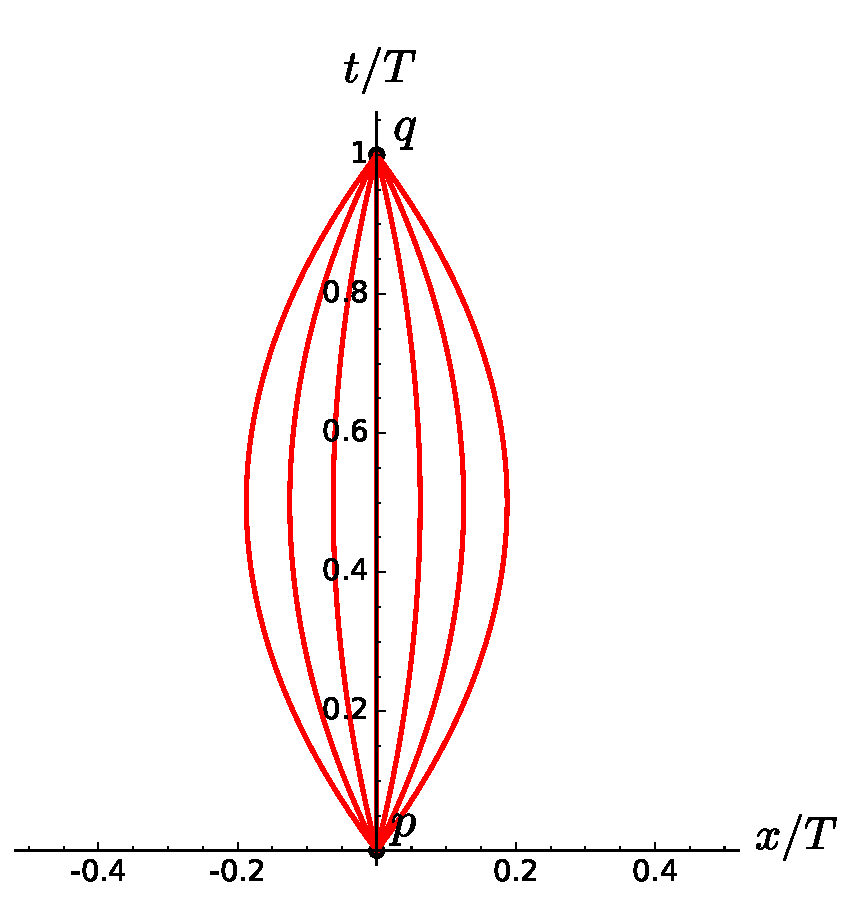
\includegraphics[height=0.3\textheight]{geo_timelike_h.pdf}}
\caption[]{\label{f:geo:timelike_h} \footnotesize
Timelike curves $\mathcal{C}_h$ connecting the point $p$
of coordinates $(0,0,0,0)$ to the point $q$ of coordinates $(T,0,0,0)$
in Minkowski spacetime. From the left to right, the depicted curves
correspond to $h$ spanning $[-3/4, 3/4]$, with the step $\delta h = 1/4$.}
\end{figure}


\begin{example}[Timelike geodesic in Minkowski spacetime] \label{x:geo:timelike_geod_Mink}
Let us suppose that $(\M,\w{g})$ is the 4-dimensional Minkowski spacetime.
All geodesics are then (segments of) straight lines. If $p$ and $q$ are
connected by a timelike geodesic $\mathcal{C}$,
we may considerer a Minkowskian coordinate system $(x^\alpha)=(t,x,y,z)$
such that $x^\alpha(p) = (0,0,0,0)$ and $x^\alpha(q) = (T,0,0,0)$, for some $T>0$.
$t$ is then the proper time along $\mathcal{C}$ and
$L_{(p,q)}(\mathcal{C})=T$. Let us consider the one-parameter family of curves
$(\mathcal{C}_h)_{h\in(-1,1)}$ defined by $x^\alpha = X^\alpha(\lambda)$ with
$\lambda\in[0,T]$ and
\[
   X^0(\lambda) = \lambda, \quad
   X^1(\lambda) = \frac{h}{T} \lambda(T - \lambda),\quad
   X^2(\lambda) = 0, \quad
   X^3(\lambda) = 0 .
\]
Note that $X^0(\lambda) = \lambda$ means that the curve parameter
coincides with the time coordinate: $\lambda = t$.
We have $\mathcal{C}_0 = \mathcal{C}$ and for $h\not=0$, $\mathcal{C}$ is
an arc of parabola connecting $p$ to $q$ in the $(t,x)$ plane
(cf. Fig.~\ref{f:geo:timelike_h}); the dimensionless
parameter $h$ is related to the curve's maximal extension along $x$ by
$x_{\rm max} = h T /4$. We have
\[
   \dot{X}^0(\lambda) = 1, \quad
   \dot{X}^1(\lambda) = h \left( 1 - 2\frac{\lambda}{T} \right),\quad
   \dot{X}^2(\lambda) = 0, \quad
   \dot{X}^3(\lambda) = 0 .
\]
Given that $(g_{\alpha\beta}) = \mathrm{diag}(-1,1,1,1)$, it follows that
$g_{\mu\nu} \dot{X}^\mu \dot{X}^\nu = -1 + h^2(1-2\lambda/T)^2$.
Since $\lambda\in[0,T]$, this shows that $\mathcal{C}_h$ is a timelike
curve as long as $-1\leq h \leq 1$. Its length is
\[
L_{(p,q)}(\mathcal{C}_h) = \int_{0}^{T} \sqrt{ 1 - h^2 \left( 1 - 2\frac{\lambda}{T} \right)^2 }
    \, \D\lambda  = \frac{T}{2h} \int_{-h}^h \sqrt{1 - u^2} \, \D u
    = \frac{T}{2h} \int_{-\mathrm{arcsin}\, h}^{\mathrm{arcsin}\, h}
        \cos^2 \theta \, \D \theta .
\]
Evaluating the integral leads to
\[
    L_{(p,q)}(\mathcal{C}_h) = \frac{T}{2} \left( \sqrt{1-h^2} + \frac{\mathrm{arcsin}\, h}{h} \right) .
\]
Note that $\mathrm{arcsin}\, h/h$ is well defined at $h=0$, since
$\lim_{h\rightarrow 0}  \mathrm{arcsin}\, h/h = 1$.
The graph of $L_{(p,q)}(\mathcal{C}_h)$ as a function $h$ is plotted in
Fig.~\ref{f:geo:timelike_length_h}. We see clearly that $h=0$, i.e. the
geodesic $\mathcal{C}$, corresponds to the maximal length.
\end{example}

\begin{figure}
\centerline{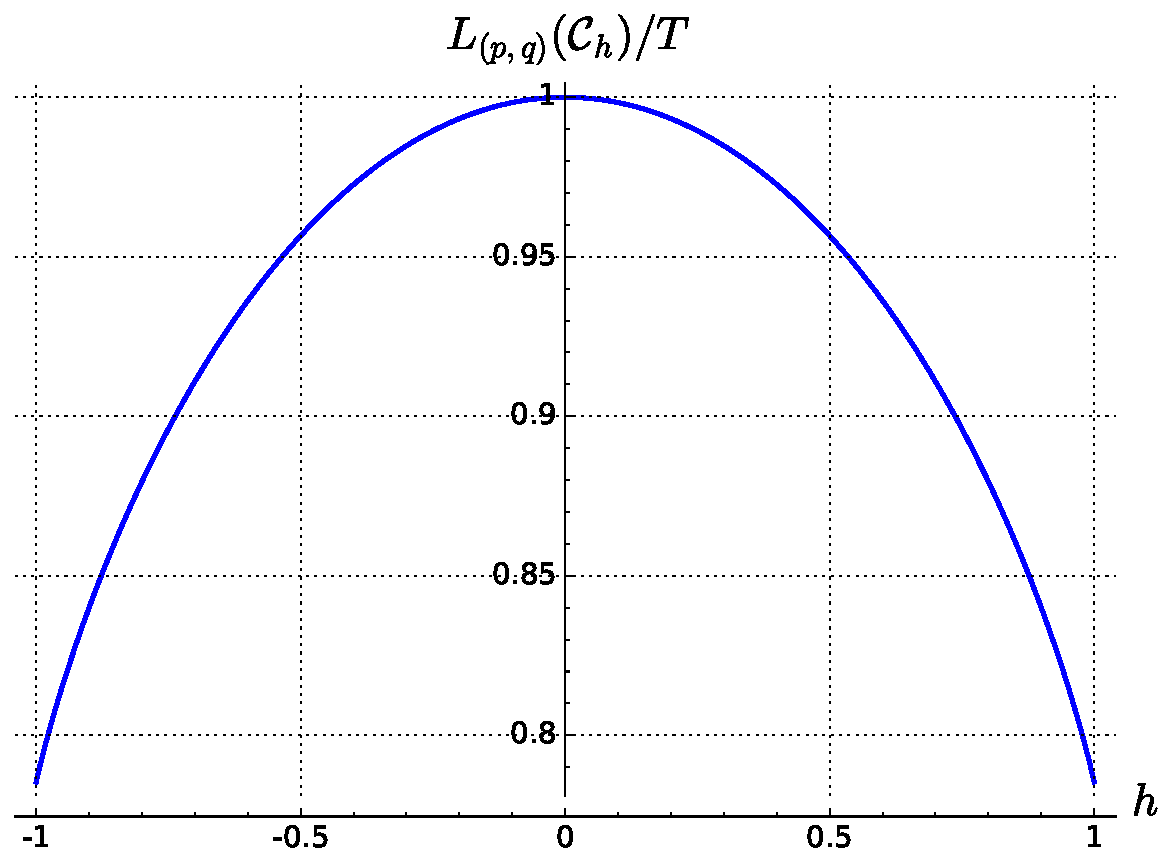
\includegraphics[height=0.3\textheight]{geo_timelike_length_h.pdf}}
\caption[]{\label{f:geo:timelike_length_h} \footnotesize
Length of the timelike curve $\mathcal{C}_h$ connecting the point $p$
of coordinates $(0,0,0,0)$ to the point $q$ of coordinates $(T,0,0,0)$
in Minkowski spacetime, as a function of the parameter $h$ measuring
the deviation from the timelike geodesic $\mathcal{C}$.}
\end{figure}


For a spacelike geodesic in a Lorentzian manifold,
the stationary length corresponds neither to a
maximum nor a minimum, but rather to a \emph{saddle point}, as the example
below illustrates.

\begin{figure}
\centerline{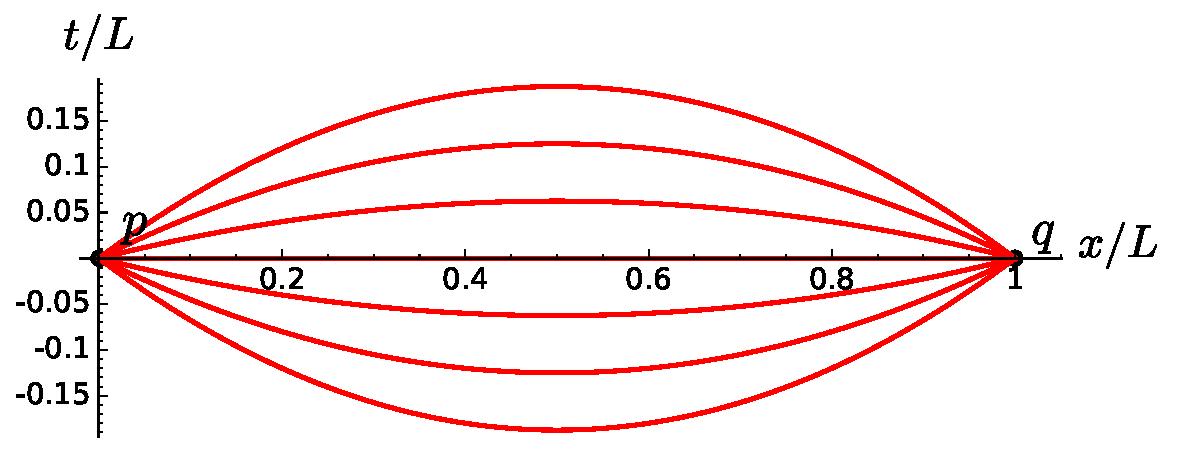
\includegraphics[width=0.7\textwidth]{geo_spacelike_h.pdf}}
\caption[]{\label{f:geo:spacelike_h} \footnotesize
Spacelike curves $\mathcal{C}_h$ connecting the point $p$
of coordinates $(0,0,0,0)$ to the point $q$ of coordinates $(0,L,0,0)$
in Minkowski spacetime. From the bottom to the top, the depicted curves
correspond to $h$ spanning $[-3/4, 3/4]$, with the step $\delta h = 1/4$.}
\end{figure}

\begin{example}[Spacelike geodesic in Minkowski spacetime]
As in Example~\ref{x:geo:timelike_geod_Mink}, we consider Minkowksi spacetime,
but this time $\mathcal{C}$ is assumed to be a spacelike geodesic connecting
two points $p$ and $q$. Since $\mathcal{C}$ is necessarily a straight line
segment, without any loss of generality, we may introduce a Minkowskian coordinate
system $(x^\alpha)=(t,x,y,z)$ such that $x^\alpha(p) = (0,0,0,0)$ and
$x^\alpha(q) = (0,L,0,0)$ for some $L>0$, which is nothing but the length
$L_{(p,q)}(\mathcal{C})$ of the geodesic $\mathcal{C}$. Any spacelike curve
$\mathcal{C}'$ connecting $p$ and $q$ and lying in the hyperplane $\Sigma$
defined by $t=0$ obeys $L_{(p,q)}(\mathcal{C}') \geq L_{(p,q)}(\mathcal{C})$
since $\Sigma$, equipped with the metric induced by $\w{g}$, is a
3-dimensional Euclidean space.

Let us consider a one-parameter family of curves
$(\mathcal{C}_h)_{h\in(-1,1)}$ lying in the orthogonal complement $\Sigma$
through $p$ and $q$, namely the curves defined $x^\alpha = X^\alpha(\lambda)$ with
$\lambda\in[0,L]$ and
\[
   X^0(\lambda) = \frac{h}{L} \lambda(L - \lambda), \quad
   X^1(\lambda) = \lambda, \quad
   X^2(\lambda) = 0, \quad
   X^3(\lambda) = 0 .
\]
As in Example~\ref{x:geo:timelike_geod_Mink}, we have $\mathcal{C}_0=\mathcal{C}$
and for $h\not=0$, the $\mathcal{C}_h$'s are
arcs of parabola connecting $p$ and $q$, which remain spacelike as long as
$-1<h<1$ (cf. Fig.~\ref{f:geo:spacelike_h}).
The computations are very similar to those of Example~\ref{x:geo:timelike_geod_Mink},
leading to
\[
    L_{(p,q)}(\mathcal{C}_h) = \frac{L}{2} \left( \sqrt{1-h^2} + \frac{\mathrm{arcsin}\, h}{h} \right) .
\]
$L_{(p,q)}(\mathcal{C}_h) / L$ is exactly the same of function of $h$
as $L_{(p,q)}(\mathcal{C}_h) / T$ in Example~\ref{x:geo:timelike_geod_Mink}.
In view of Fig.~\ref{f:geo:timelike_length_h}, we therefore assert
that $L_{(p,q)}(\mathcal{C}_h) \leq L_{(p,q)}(\mathcal{C})$.

We conclude that the spacelike geodesic $\mathcal{C}$ corresponds to a
saddle point of the length functional: it is a minimum among the curves lying
in the $(x,y,z)$ hyperplane but a maximum among those lying in the $(t,x)$
plane.
\end{example}


%%%%%%%%%%%%%%%%%%%%%%%%%%%%%%%%%%%%%%%%%%%%%%%%%%%%%%%%%%%%%%%%%%%%%%%%%%%%%%%


\section{Geodesics and symmetries}













